%%%%%%%%%%%%%%%
%
% $Autor: Wings $
% $Datum: 2020-01-29 07:55:27Z $
% $Pfad: General/SensorBME280.tex
% $Version: 1785 $
%
%
%%%%%%%%%%%%%%%

%todo   url       = {https://lastminuteengineers.com/bme280-arduino-tutorial/},


	
\chapter{Sensor BME280 für Temperatur, Luftfeuchtigkeit und den Luftdruck}

\section{Beschreibung der Hardware}

Der BME280 ist ein Temperatursensor, der von Bosch Sensortec entwickelt wurde. Der Sensor bietet die Möglichkeit, die Temperatur, Luftfeuchtigkeit und den Luftdruck in der Umgebung zu messen, siehe Abbildung \ref{fig:SensorBME280}). \cite{FunduinoBME280:2023}

\begin{figure}[h]
    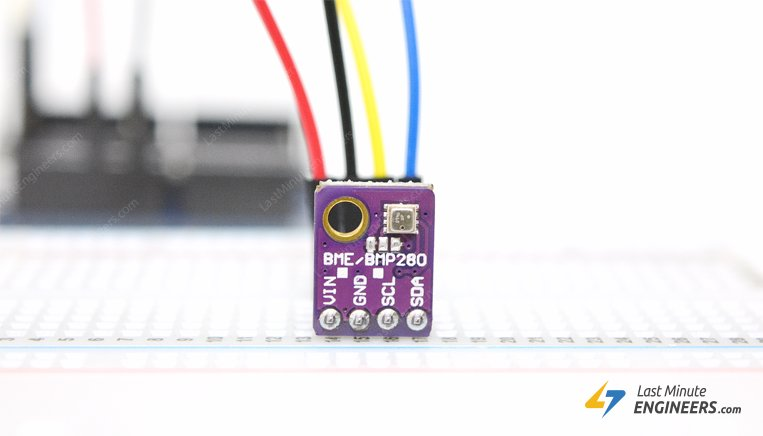
\includegraphics[width=\textwidth]{Sensor/BMEsensor}
    \caption{Sensor BME280}   \cite{LastMinuteEngineers:2023}
    \centering   \label{fig:SensorBME280}
\end{figure}

Bei dem BME280 handelt es sich um einen kombinierten Sensor für die Messung von Feuchtigkeit, Luftdruck und Temperatur. Dieser ist auf dem Entwicklerboard DEBO BME280 verbaut. Das Entwicklerboard hat die Maße 15,3 x 11,5 x 2,5 mm (LxBxH), wobei der Sensor BME280 die Maße 2,5 x 2,5 x 0,93 mm (LxBxH) aufweist. Die Schnittstellen I2C und SPI des Entwicklerboards ermöglichen die Kommunikation zwischen dem Arduino und dem Sensor. Die Versorgungsspannung bewegt sich zwischen 1,72 V und 3,6 V. Die gemessene Luftfeuchtigkeit erfolgt mit einer Genauigkeitstoleranz von $\pm 3$ Prozent relativer Luftfeuchtigkeit und einer Reaktionszeit von einer Sekunde. Der Druckbereich für den Luftdruck beträgt 300 bis 1100 hPa mit einer relativen Genauigkeit von $\pm 0.12$ hPa und einer absoluten Genauigkeiten von $\pm 1$ hPa. Der Temperatursensor hat einen Bereich von -40 bis +85 °C und besitzt eine voll Genauigkeit im Bereich von $0^\circ$ bis $65^\circ$ C. Der durchschnittliche Stromverbrauch des Sensors bei einer Frequenz von 1 Hz beträgt $1.8 \mu$A für die Messung von Feuchtigkeit und Temperatur, $2.8\mu$A für die Messung von Luftdruck und Temperatur und $3.6\mu$A für die Messung von Feuchtigkeit, Luftdruck und Temperatur. Der Sensor BME280 verfügt über mehrere Pins, die für verschiedene Zwecke verwendet werden. Hierbei ist es wichtig die richtige Pin-Belegung für den Sensor zu kennen. Im Allgemeinen sind die Pins wie folgt belegt: Der VCC-Pin wird mit der positiven Stromversorgung (+3.3 V oder +5 V) des Systems verbunden. Der GND-Pin muss mit dem Masseanschluss (GND) Ihres Systems verbunden werden. Der SDA-Pin ist der Datenpin für die Kommunikation I2C. Dieser wird mit dem entsprechenden SDA-Pin auf dem Mikrocontroller verbunden. Der SCL-Pin ist der Takt-/Clock-Pin für die Kommunikation I2C. Dieser muss mit dem entsprechenden SCL-Pin auf dem Mikrocontroller verbunden werden. SDI sorgt für die SPI-Kommunikation. \cite{Bosch:2015,Bosch:2021}


\section{Schaltplan des Aufbaus}

Der folgende Schaltplan stellt die Komponenten des Arduino Nano BLE Sense Lite, des Sensors BME280 und des OLED-Displays dar. Als Spannungsquelle dient ein Computer, der den Arduino Nano 33 BLE Sense über ein USB-A auf Mikro-USB Kabel versorgt. Die Komponenten sind sinngemäß miteinander verbunden und in Abbildung~\ref{fig:Schaltplan} abgebildet.

\begin{figure}[h]
    \centering
    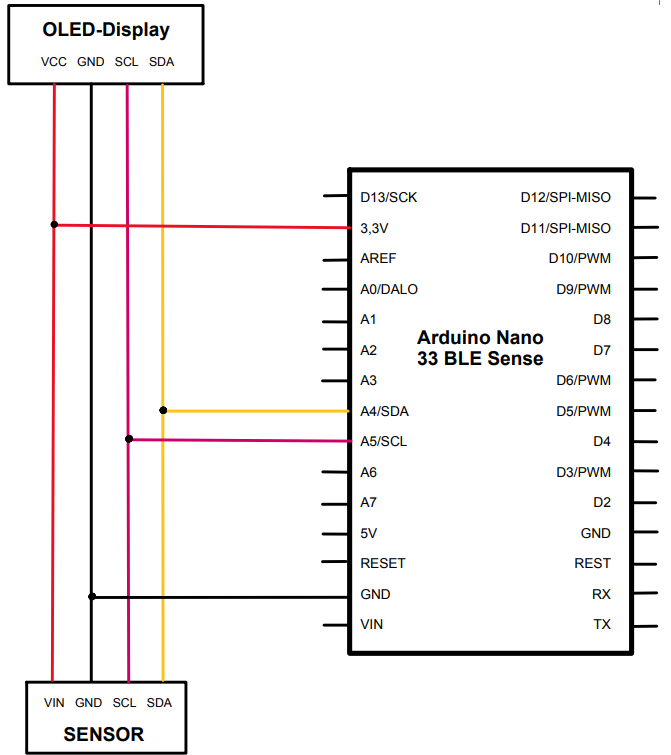
\includegraphics[width=0.5\textwidth] {Sensor/BMECircuit}
    \caption{Stationärer Aufbau der Wetterstation}
    \label{fig:Schaltplan} \cite{ArduinoNano33Manual:2022}
\end{figure}

\subsection{Bibliothek \FILE{cactus\_io\_BME280} für den Sensor BME280}

Die Bibliothek \FILE{cactus\_io\_BME280\_I2C} ist eine spezielle Arduino Bibliothek zur Kommunikation mit dem Sensor BME280. Die Bibliothek erleichtert die Interaktion mit dem Sensor BME280 und bietet eine einfache Möglichkeit, Messwerte abzurufen und sie in Ihren Arduino-Projekten zu verwenden. Um die Bibliothek \FILE{cactus\_io\_BME280\_I2C} zu verwenden, muss sie erst als ZIP-Datei heruntergeladen und anschließend von dem Arduino Library Manager installiert werden. Mit Hilfe von \PYTHON{\#include<"cactus\_io\_BME280\_I2C">} können diese in dem Arduino-Code eingebunden werden. \cite{IotSpace:2020}

\subsection{Testen des OLED-Displays}

Für die Programmierung des Displays gibt es viele Möglichkeiten. Da es viele Librarys gibt, muss zuerst einmal überlegt werden, welche verwendet werden sollen. Um einen ersten Eindruck über die Programmierung des Displays zu bekommen, wurde zunächst ein Beispielsketch getestet. Es handelt sich hier um den Sketch ``Hello World'', welcher unter \FILE{Datei -> SSD1206Ascii -> HelloWorldWire} zu finden ist (siehe Abbildung~\ref{fig:TestprogrammDisplay}).

\begin{figure}
  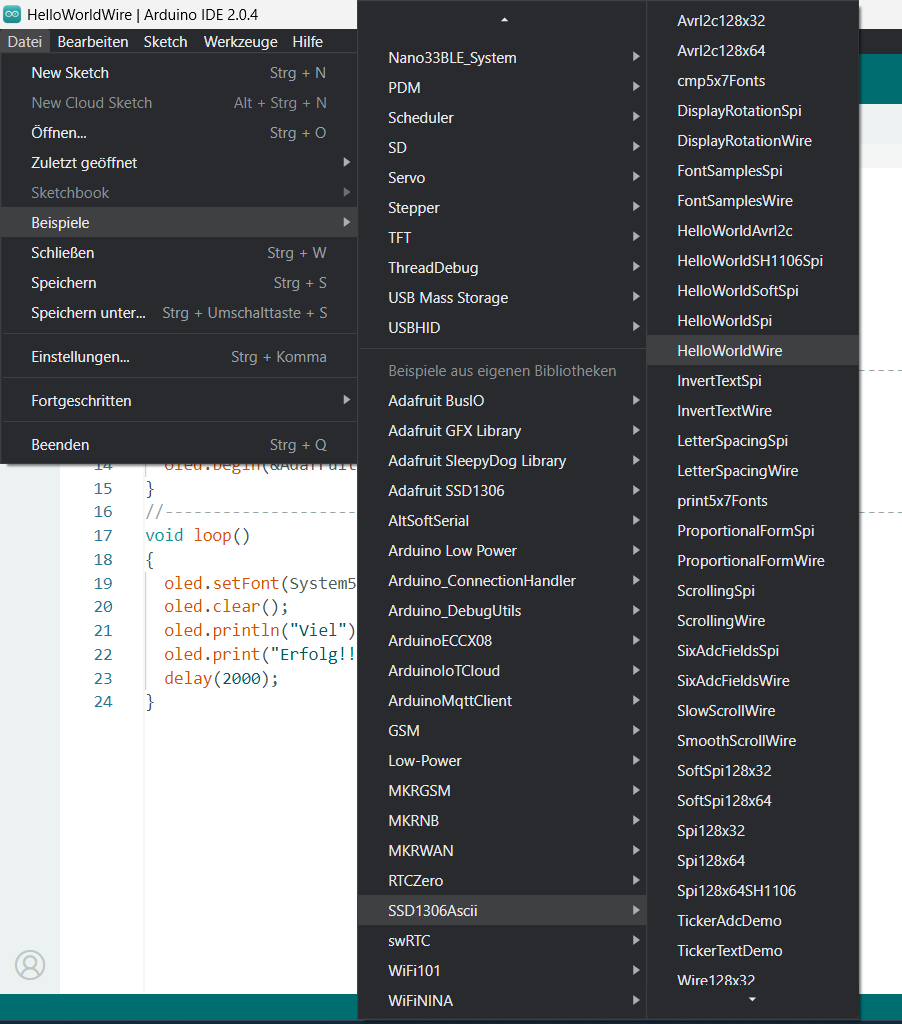
\includegraphics[width=1\textwidth]{OLED/TestprogrammDisplay}
  \caption{Pfad des Testprogramms.}
  \label{fig:TestprogrammDisplay}
\end{figure}

Das Testprogramm ``Hello World''(siehe Seite \pageref{Test1}) wird dafür benutzt, um den Text Hello World auf dem Display auszugeben (siehe Abbildung \ref{fig:ErsteAusgabeDisplay}). Es wird hier verwendet, um sich mit der Software vertraut zu machen und um sicherzustellen, dass die Entwicklungsumgebung richtig eingerichtet ist. Außerdem wird getestet, ob das Programmieren funktioniert und alle Kabel richtig angesteckt sind.

\bigskip

\begin{code}
\begin{Arduino}
#include <Wire.h>
#include ``SSD1306Ascii.h''
#include ``SSD1306AsciiWire.h''
#define I2C_ADDRESS 0x3c

SSD1306AsciiWire oled;

void setup() 
{
  Wire.begin();
  Wire.setClock(400000L);
  oled.begin(\&Adafruit128x64, I2C\_ADDRESS);
}

void loop()
{
  oled.setFont(System5x7);
  oled.clear();
  oled.println(``Viel'');
  oled.print(``Erfolg!!!'');
  delay(2000);
}
\end{Arduino}\label{Test1}
  \caption{Testprogramm für ein OLED-Display}
\end{code}


Nachdem der Quellcode kompiliert und an den Arduino geschickt wurde, wurde auf dem Display der Text Viel Erfolg ausgegeben (siehe Abbildung \ref{fig:ErsteAusgabeDisplay}). Hiermit ist sichergestellt worden, dass die Entwicklungsumgebung und der Compiler korrekt funktionieren. \Mynote{citation}

\begin{figure}
  \centering
  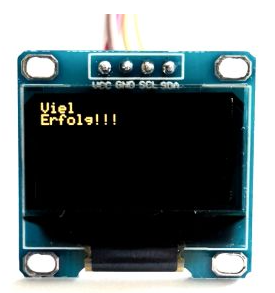
\includegraphics[width=0.5\textwidth] {OLED/Output}
  \caption{Erste Ausgabe Display} 
  \label{fig:ErsteAusgabeDisplay} \Mynote{citation}
\end{figure}

